\documentclass[11pt,aspectratio=169]{beamer}
% Deliberately simple: default theme, no Metropolis (matches the primer deck).
\usetheme{default}
\usecolortheme{dove}
\usefonttheme{serif}
\setbeamertemplate{navigation symbols}{}
\setbeamertemplate{footline}{}
\setbeamertemplate{itemize items}[circle]

\usepackage{amsmath,amssymb}
\usepackage{booktabs}
\usepackage{graphicx}
\usepackage{xcolor}
\usepackage[most]{tcolorbox}
\usepackage{minted}
\usemintedstyle{friendly}                 % colorful pygments theme
\setminted{fontsize=\scriptsize,breaklines,autogobble,tabsize=2,escapeinside=||}
\setminted[cpp]{fontsize=\scriptsize}
\setminted[python]{fontsize=\scriptsize}

\graphicspath{{figs/}{../paper/figures/}{../figs/}}

\definecolor{key}{rgb}{0.10,0.35,0.65}
\newcommand{\bhat}{\hat{\mathbf{b}}}
\setbeamercolor{frametitle}{fg=key}
% small manual footnote (no marker collisions)
\newcommand{\notefoot}[1]{\vfill{\footnotesize #1\par}}

\title{A Native Spin-Polarized Neutron Source in OpenMC}
\subtitle{From \texttt{TokamakSource} to a 3-D Equilibrium \texttt{StellaratorSource}}
\author{Thaddaeus Kiker}
\date{\today}

\begin{document}
\frame{\titlepage}

% ============================================================
\begin{frame}{Miscellaneous Updates}
\begin{itemize}
\item Scheduling a meeting with Dr.\ Elizabeth Paul (Columbia) to discuss quasi-symmetry
      and stellarator optimization, and how her equilibrium/QS expertise could inform the
      QUASR device selection and equilibrium inputs feeding this source.
\item My apartment building caught on fire yesterday (photos follow).
\end{itemize}
\end{frame}

\begin{frame}{Miscellaneous Updates}
\centering
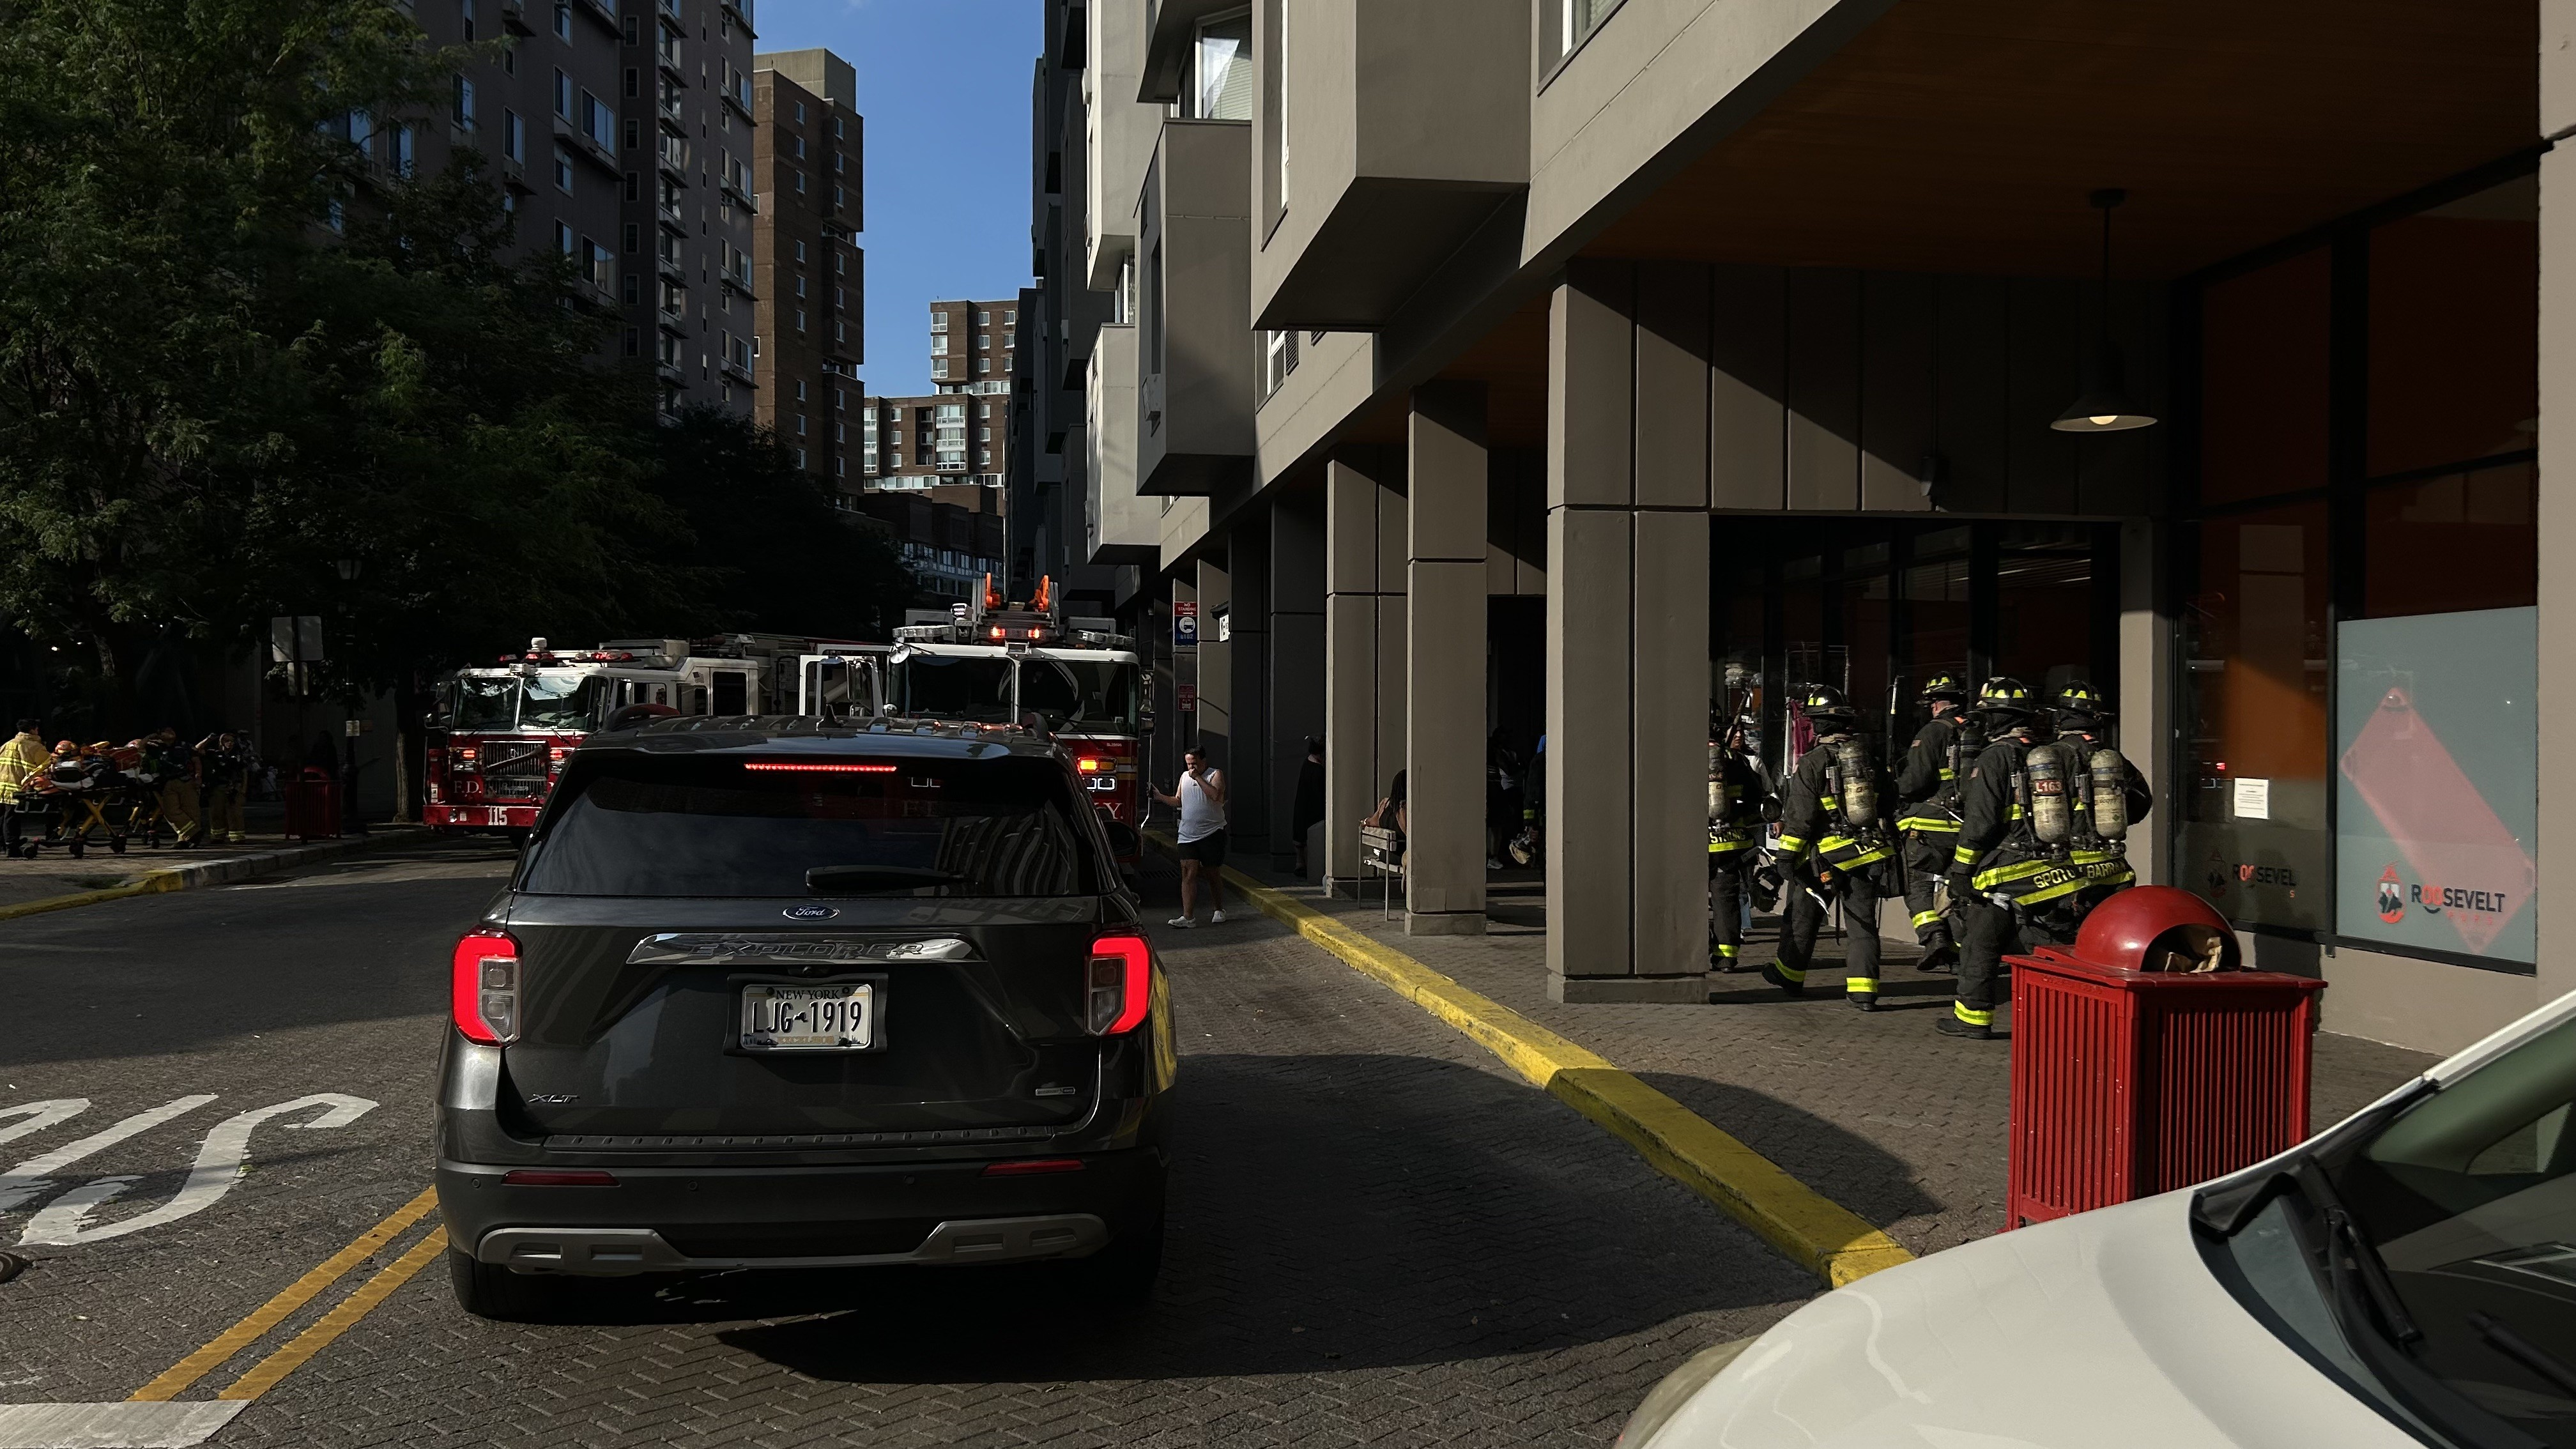
\includegraphics[width=0.92\linewidth]{misc_fire1.jpg}
\end{frame}

\begin{frame}{Miscellaneous Updates}
\centering
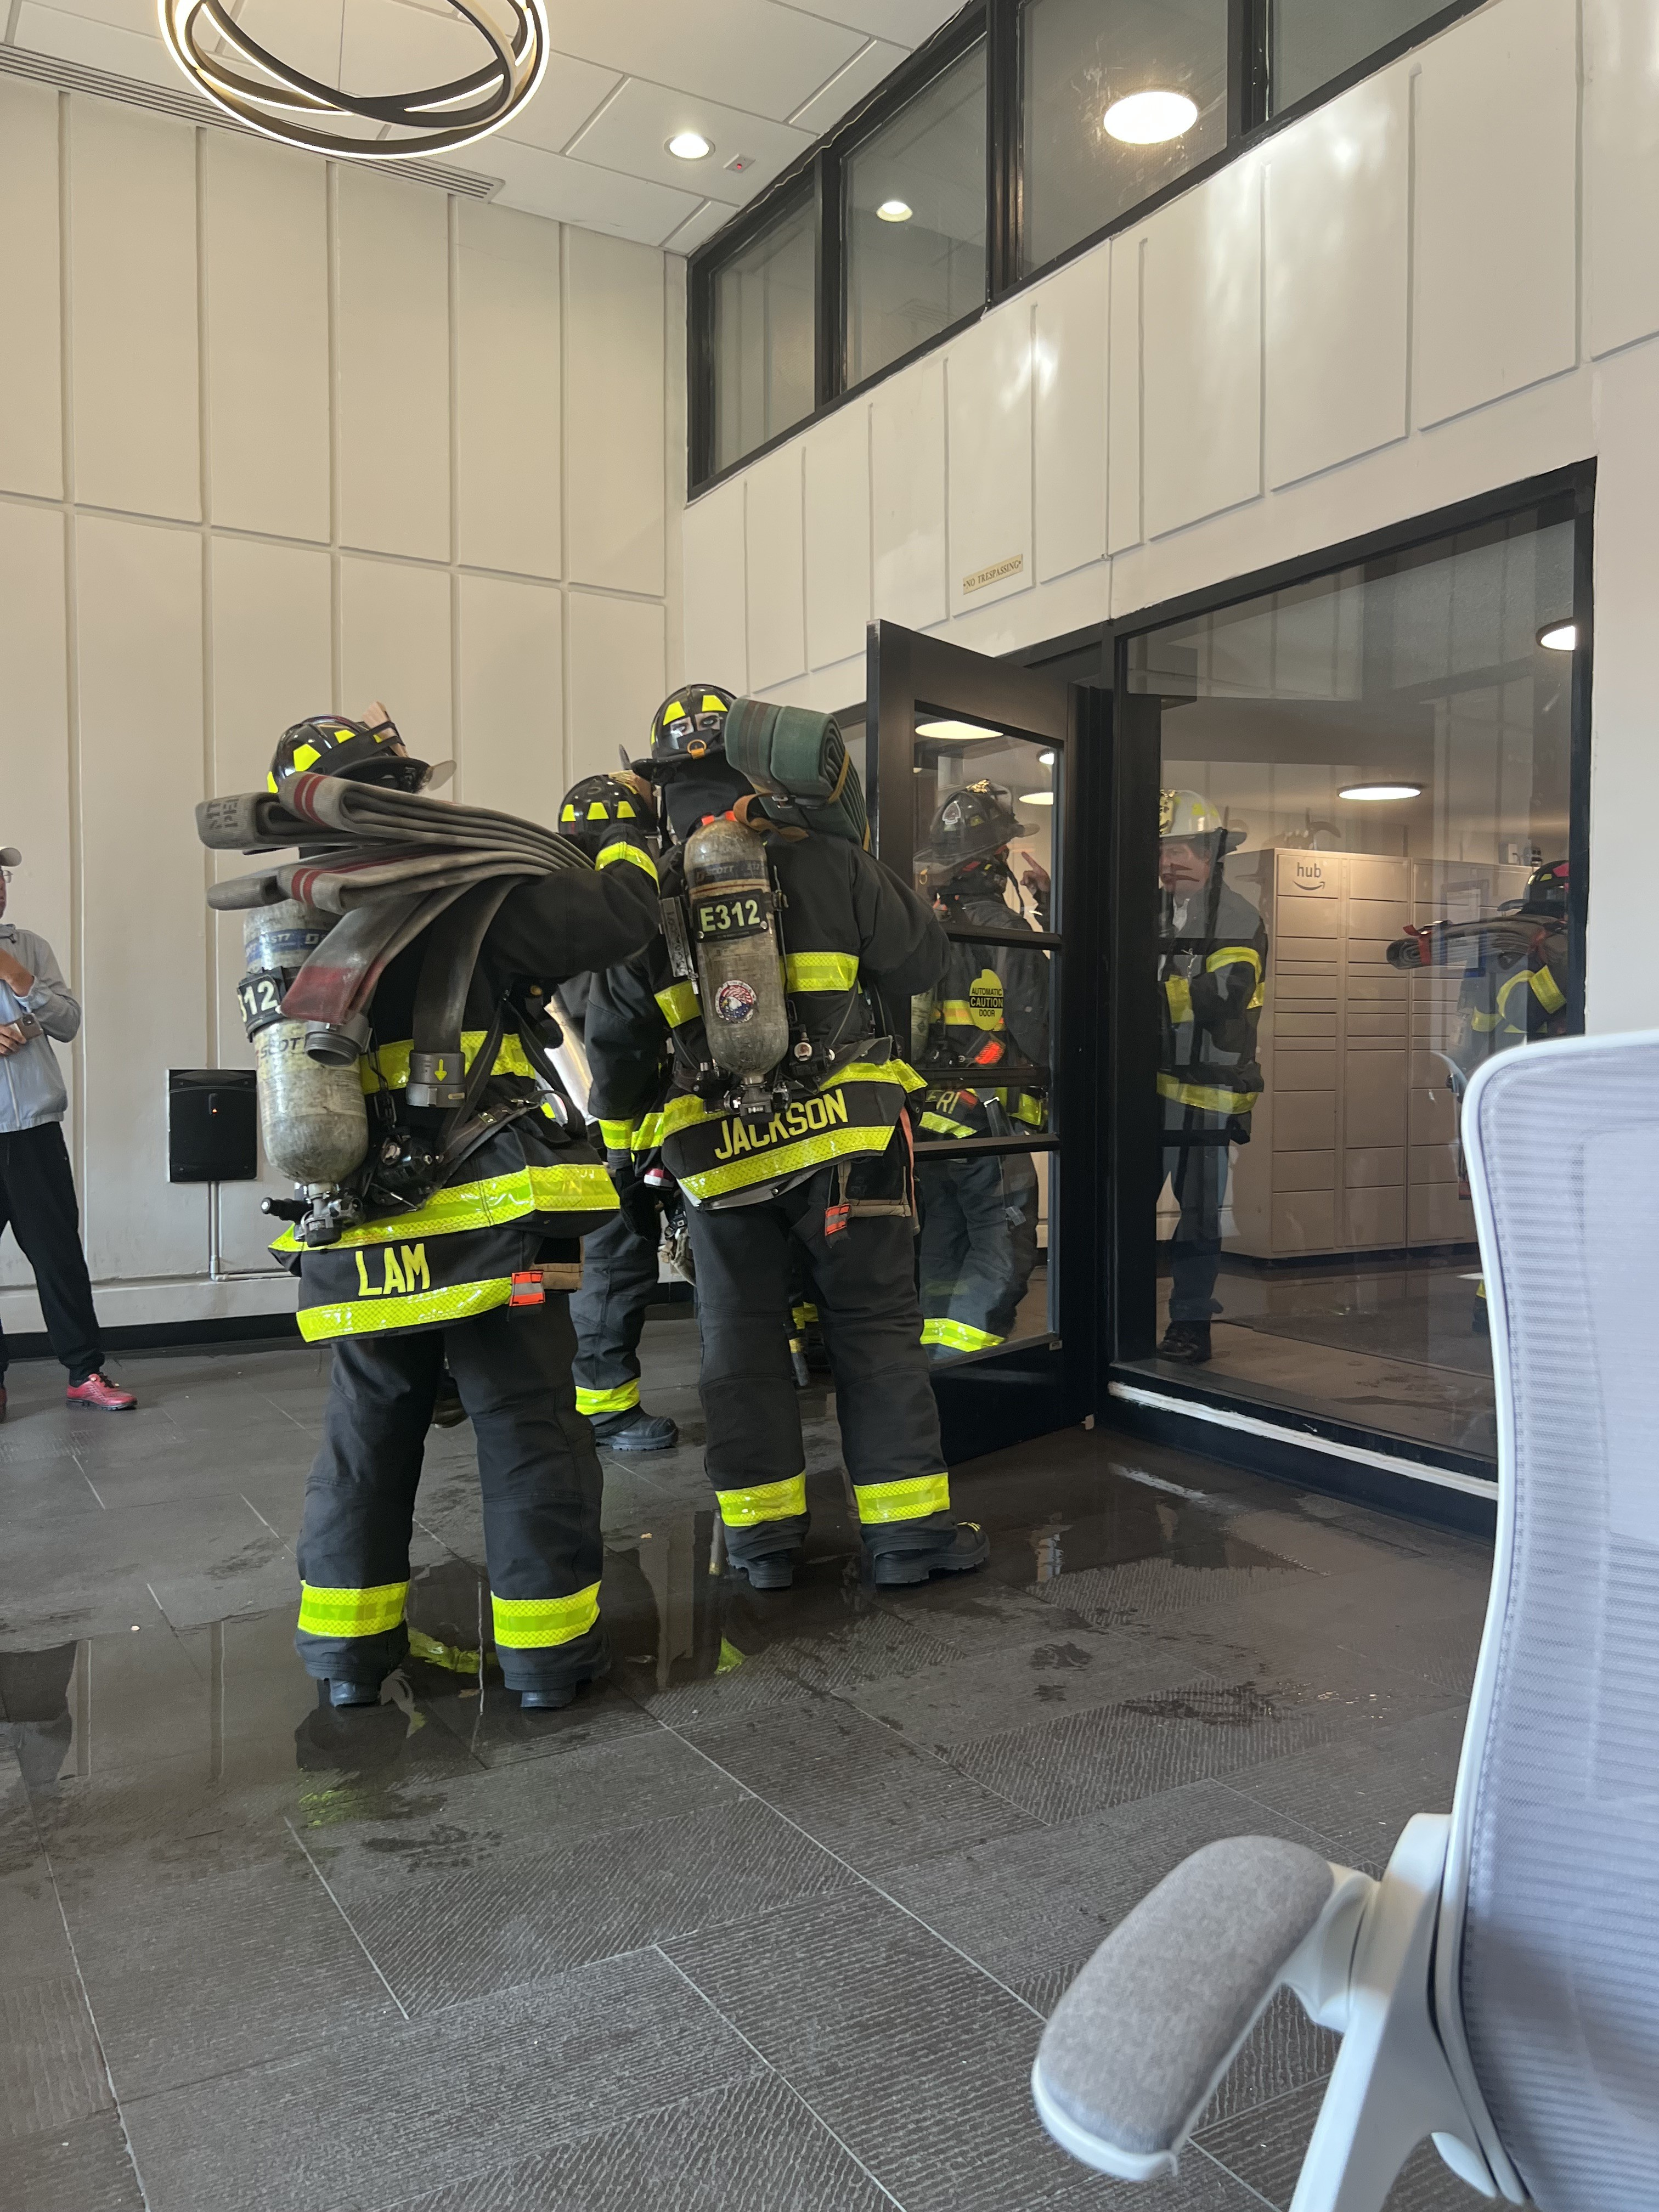
\includegraphics[height=0.84\textheight]{misc_fire2.jpg}
\end{frame}

% ============================================================
\begin{frame}{What I Built This Week}
\begin{itemize}
\item A native OpenMC C++ \texttt{Source} subclass that samples spin-polarized D--T
      neutron emission in the local field frame, driven by a real 3-D equilibrium flux
      map (DESC/VMEC).\footnote{\scriptsize A precomputed, tabulated OpenMC tokamak
      neutron source also exists (Bae et al., Nucl.\ Fusion 65, 086051, 2025); it bakes
      the emission into a fixed sampled distribution rather than generating it natively on
      the fly, so it cannot carry the local-field-dependent polarized direction.}
\item Built on the \texttt{TokamakSource} pattern (PR \#3999): the same rejection-free CDF
      cascade and native-\texttt{Source} plumbing.
\item Adds polarized emission about $\bhat$, real equilibrium geometry with $\sqrt{g}$
      weighting, and genuine three-dimensionality.
\item Verified against analytic theory, cross-checked on real QUASR geometry, and run
      end-to-end through a conformal multi-material blanket.
\end{itemize}
\end{frame}

% ============================================================
\begin{frame}{Lineage}
\begin{itemize}
\item \texttt{source.cpp.orig}: your \texttt{TokamakSource} (PR \#3999). Parametric
      Miller geometry, rejection-free cascade in $(r/a,\alpha,\phi)$, isotropic emission.
\item \texttt{source.cpp}: my SPF patch to that class. Added the polarized-direction
      machinery (\texttt{sample\_polarized\_direction}, \texttt{field\_model}, the
      $(a,b,c)\!\to\!w_\perp,w_\parallel$ mixture).
\item \texttt{stellarator\_source.cpp}: the new class. Same direction sampler, but geometry
      comes from a real equilibrium flux map with $\sqrt{g}$ weighting and a gridded 3-D
      $\bhat$.
\end{itemize}
\notefoot{$\dagger$~Note: my prototype emits monoenergetic 14.06\,MeV, whereas your
\texttt{TokamakSource} supports per-$r$ energy spectra.}
\end{frame}

% ============================================================
\begin{frame}{TokamakSource vs StellaratorSource}
\scriptsize
\begin{tabular}{@{}p{2.3cm}p{4.4cm}p{4.6cm}@{}}
\toprule
 & \texttt{TokamakSource} (PR \#3999) & \texttt{StellaratorSource} (new) \\
\midrule
Geometry & analytic parametric Miller $(R_0,a,\kappa,\delta,\Delta)$ & real DESC/VMEC
   equilibrium flux map (\texttt{spf\_fluxmap\_v1}) \\
Position & rejection-free cascade $p(r/a)\!\to\!p(\alpha|r)\!\to\!\phi$; analytic
   \texttt{flux\_to\_cartesian} & rejection-free cascade $\rho\!\to\!\zeta\!\to\!\theta$,
   weight $S(\rho)\,|\sqrt{g}|$; trilinear interp of $R,Z,\phi$ \\
Emission & isotropic only & polarized $P_2$ mixture about local $\bhat$ \\
Field & none & \texttt{fluxmap} (gridded $B_R,B_\phi,B_Z$) or \texttt{toroidal}
   ($\hat\varphi$, axisymmetric-limit gate) \\
Dimension & axisymmetric & genuinely 3-D non-axisymmetric \\
Core & C++ \texttt{Source} & C++ \texttt{Source} (line-for-line port of a validated
   Python reference) \\
\bottomrule
\end{tabular}
\end{frame}

% ============================================================
\begin{frame}{The Physics (Schwartz 2025)}
Aligned D--T spins make the 14.1\,MeV neutron emission anisotropic about the local field
$\bhat$:
\only<1>{\[
\frac{d\sigma}{d\Omega} = \frac{\sigma_0}{2\pi}\Big[\tfrac34\,a\,\sin^2\theta
 + \big(\tfrac23 b + \tfrac13 c\big)\big(\tfrac14 + \tfrac34\cos^2\theta\big)\Big],
\qquad \theta = \angle(\mathbf{u},\bhat).
\]}
\only<2->{\[
\frac{d\sigma}{d\Omega} = \frac{\sigma_0}{2\pi}\Big[
 \underbrace{\tfrac34\,a\,\sin^2\theta}_{\text{perp shape}}
 + \underbrace{\big(\tfrac23 b + \tfrac13 c\big)\big(\tfrac14 + \tfrac34\cos^2\theta\big)}_{\text{parallel shape}}\Big],
\qquad \theta = \angle(\mathbf{u},\bhat).
\]}
\onslide<2->{Two shapes, so two weights plus a scalar rate:
\[
w_\perp = \tfrac34 a, \qquad
w_\parallel = \tfrac23 b + \tfrac13 c, \qquad
\eta = a + \tfrac23 b + \tfrac13 c.
\]}
\onslide<3->{
\begin{itemize}\footnotesize
\item A $(1,0,0)$: $\sin^2\theta$, perpendicular, $\eta=1$ ($+50\%$ rate).
\item B $(0,1,0)$: $\tfrac14+\tfrac34\cos^2\theta$, parallel, $\eta=\tfrac23$ (same rate as
      unpolarized).
\item C $(0,0,1)$: same shape as B, $\eta=\tfrac13$ (half rate); not isotropic.
\item Unpolarized $(\tfrac13,\tfrac13,\tfrac13)$: $\eta=\tfrac23$; NWL exactly linear in
      $a_2$.
\end{itemize}}
\end{frame}

% ============================================================
\begin{frame}[fragile]{Constructor: Weights Derived, Not Pasted}
The $(a,b,c)$ input becomes two weights plus a selection probability. The integrals
$\int\sin^2\theta\,d\Omega = 8\pi/3$ and $\int(\tfrac14+\tfrac34\cos^2\theta)\,d\Omega = 2\pi$
give $P_\perp = a/\eta$.
\begin{minted}{cpp}
auto abc = get_node_array<double>(node, "polarization");
double a = abc[0], b = abc[1], c = abc[2];
const double s = a + b + c;
a /= s; b /= s; c /= s;

w_perp_ = 0.75 * a;
w_par_  = (2.0/3.0)*b + (1.0/3.0)*c;
const double eta = a + (2.0/3.0)*b + (1.0/3.0)*c;
p_perp_ = a / eta;
polarized_ = true;
\end{minted}
\end{frame}

\begin{frame}[fragile]{The Two Shapes: Closed-Form Inverse CDFs}
Each shape's $\cos\theta$ marginal is a cubic; both roots are closed form (no rejection).
\begin{minted}{cpp}
inline double spf_costheta_perp(double u) {          // p(x) ~ 1 - x^2
  double x = 2.0*std::cos(std::acos(1.0 - 2.0*u)/3.0 - 2.0*PI/3.0);
  return std::clamp(x, -1.0, 1.0);
}
inline double spf_costheta_par(double u) {           // p(x) ~ 1/4 + 3/4 x^2
  const double q  = 2.0 - 4.0*u;
  const double sq = std::sqrt(q*q/4.0 + 1.0/27.0);
  double x = std::cbrt(-q/2.0 + sq) + std::cbrt(-q/2.0 - sq);
  return std::clamp(x, -1.0, 1.0);
}
\end{minted}
\footnotesize These match the Python reference bit-for-bit on a fixed seed sequence
(both use libm \texttt{cbrt}).
\end{frame}

\begin{frame}[fragile]{\texttt{sample()}: Position From The Equilibrium}
Three \texttt{prn} draws walk the CDF cascade; $\sqrt{g}$ makes it a true volumetric source.
\begin{minted}{cpp}
int  i = upper_bound_strided(cdf_rho_.data(), nr_+1, 1, prn(seed)) - 1;
int kk = upper_bound_strided(&cdf_zeta_[idxZ(i,0)], nz_+1, 1, prn(seed)) - 1;
int  j = upper_bound_strided(&cdf_theta_[idxT(i,0,kk)], nt_+1, nz_, prn(seed)) - 1;

const double rr = rho_[i] + (prn(seed)-0.5)*drho_;   // jitter inside the cell
const double tt = theta_[j] + (prn(seed)-0.5)*dtheta_;
const double zz = zeta_[kk] + (prn(seed)-0.5)*dzeta_;
// trilinear interp of the stored geometry -> Cartesian:
const double R = interp(R_, ...), Z = interp(Z_, ...), PH = interp(phi_, ...);
site.r = {R*std::cos(PH), R*std::sin(PH), Z};
\end{minted}
The cascade weight is the one line that upgrades the tokamak version:
\begin{minted}{cpp}
w[idx3(i,j,kk)] = S_[i] * sqrtg_[idx3(i,j,kk)];      // emission x metric Jacobian
\end{minted}
\end{frame}

\begin{frame}[fragile]{\texttt{sample()}: Polarized Direction About $\bhat$}
Stratified pick of a shape, then a numerically safe rotation into the global frame.
\begin{minted}{cpp}
double x;
if (prn(seed) < p_perp_) x = spf_costheta_perp(prn(seed));   // sin^2 shape
else                     x = spf_costheta_par(prn(seed));    // 1/4+3/4cos^2 shape
const double az = 2.0*PI*prn(seed);
const double st = std::sqrt(std::max(0.0, 1.0 - x*x));
const Direction local{st*std::cos(az), st*std::sin(az), x};

Direction b = bhat / bhat.norm();                            // Gram-Schmidt frame
const double ax=std::abs(b.x), ay=std::abs(b.y), az2=std::abs(b.z);
Direction ref = (ax<=ay && ax<=az2) ? Direction{1,0,0}
              : (ay<=az2)           ? Direction{0,1,0} : Direction{0,0,1};
Direction ex = ref - b.dot(ref)*b; ex /= ex.norm();
Direction ey = b.cross(ex);
return (local.x*ex + local.y*ey + local.z*b).normalized();   // |u| = 1
\end{minted}
\footnotesize Least-aligned reference axis avoids the $\bhat\parallel\hat z$ degeneracy.
\end{frame}

\begin{frame}[fragile]{Python API And The Flux-Map Format}
The user-facing side stays OpenMC-idiomatic:
\begin{minted}{python}
from openmc import StellaratorSource

src = StellaratorSource(
    fluxmap="quasr59509_cm_fluxmap",     # spf_fluxmap_v1 grid
    polarization=(1.0, 0.0, 0.0),        # (a, b, c); A-mode = perpendicular
    field_model="fluxmap",               # local b-hat from the equilibrium
    energy=openmc.stats.Discrete([14.06e6], [1.0]),
)
\end{minted}
\texttt{spf\_fluxmap\_v1}: a \texttt{.meta} text header (\texttt{magic},
$n_R,n_\theta,n_\zeta,n_{fp}$) plus a little-endian f8 payload in C-order:
\[
\rho,\ \theta,\ \zeta,\ \sqrt{g},\ R,\ Z,\ \phi,\ B_R,\ B_\phi,\ B_Z .
\]
Spin fractions map in cleanly: \texttt{a=d+t+ + d-t-},\ \ \texttt{b=d0},\ \
\texttt{c=d+t- + d-t+}.
\end{frame}

% ============================================================
\begin{frame}{Verification: The Sampler Is Exact Before Any Transport}
\scriptsize
\begin{columns}[T]
\begin{column}{0.52\textwidth}
$\cos\theta$ distribution, $N=10^6$, $\chi^2$/dof (p):
\begin{tabular}{@{}lcc@{}}
\toprule
mode & $\chi^2$/dof & p \\
\midrule
unpolarized & 0.97 & 0.52 \\
A (perp) & 1.32 & 0.084 \\
B (par) & 0.75 & 0.88 \\
C & 1.37 & 0.062 \\
mixed $(.5,.3,.2)$ & 0.70 & 0.92 \\
\midrule
$\phi$ uniformity & 1.03 & 0.41 \\
isotropy-under-rotation & 0.99 & 0.54 \\
\bottomrule
\end{tabular}
\end{column}
\begin{column}{0.46\textwidth}
Inverse-CDF vs rejection (KS):\\
\quad $\sin^2\theta$: $D=3.1\!\times\!10^{-3}$, p$=0.10$\\
\quad $\tfrac14+\tfrac34\cos^2$: $D=1.8\!\times\!10^{-3}$, p$=0.69$\\[1em]
Emission moment $\langle(\mathbf{u}\!\cdot\!\bhat)^2\rangle$
(measured / analytic, 3-D field):\\
\quad unpolarized\ \ 0.3328 / 0.3333\\
\quad perp\ \ \ 0.2007 / 0.2000\\
\quad par\ \ \ \ 0.4668 / 0.4667\\[1em]
All gates pass. The $a_2$-linearity identity
$\mathrm{NWL}_\perp+\mathrm{NWL}_\parallel = 2\,\mathrm{NWL}_{\text{unpol}}$
holds to statistics.
\end{column}
\end{columns}
\end{frame}

% ============================================================
\begin{frame}{The Conformal Multi-Material Blanket (1/2)}
\begin{columns}[c]
\begin{column}{0.62\textwidth}
\includegraphics[width=\linewidth]{wall_cutaway.pdf}
\end{column}
\begin{column}{0.36\textwidth}
\footnotesize
Radial build offset outward from the VMEC LCFS:
\begin{itemize}
\item W\ \ 0.2\,cm
\item Steel\ \ 3.8\,cm
\item Be\ \ 2.0\,cm
\item FLiBe\ \ 50\,cm
\item Shield\ \ 40\,cm
\item Coil\ \ 15\,cm
\end{itemize}
Device scaled $\times10$ to reactor size. Non-convex bean cross-sections handled directly.
\end{column}
\end{columns}
\end{frame}

\begin{frame}{The Conformal Multi-Material Blanket (2/2)}
\footnotesize
\begin{itemize}
\item Each layer surface is the LCFS offset along its poloidal outward normal by the
      cumulative thickness (\texttt{offset\_surface} in \texttt{stellarator\_geometry.py}).
\item Built as watertight shell-solid STLs, one per layer, then combined into a DAGMC
      \texttt{.h5m} that OpenMC transports through directly, with non-convex-safe meshing
      so the bean-shaped QA cross-sections close without self-intersection.
\item Materials: W plasma-facing armor, RAFM steel first wall, Be neutron multiplier,
      FLiBe tritium breeder, WC/steel shield, coil pack.
\item Thicknesses are representative fusion-blanket values (thin plasma-facing armor,
      cm-scale steel/multiplier, $\sim\!0.5$\,m breeder, $\sim\!0.4$\,m shield, coil
      pack).
\end{itemize}
\end{frame}

% ============================================================
\begin{frame}{End-To-End: Transported Flux And Heating}
\begin{columns}[c]
\begin{column}{0.6\textwidth}
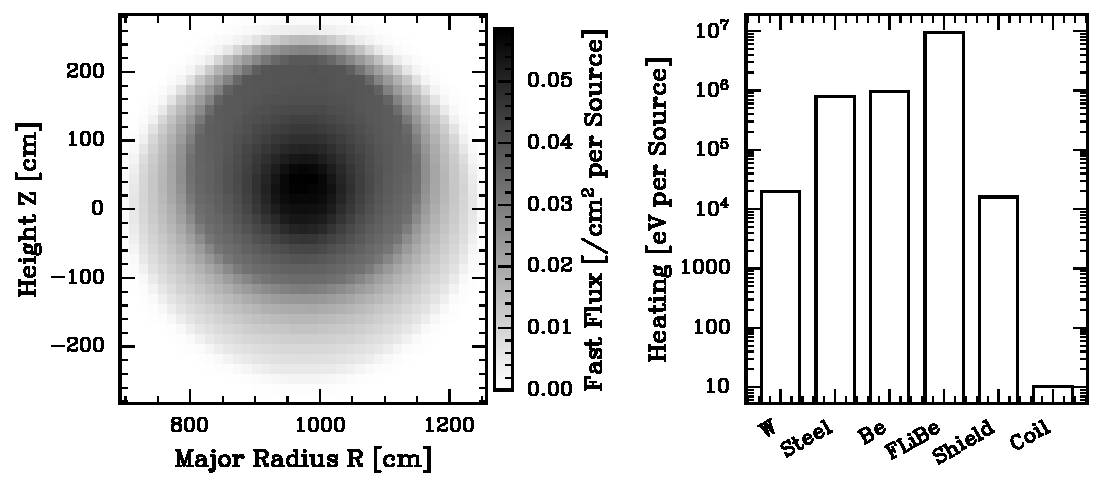
\includegraphics[width=\linewidth]{fig_conformal_flux.pdf}
\end{column}
\begin{column}{0.38\textwidth}
\footnotesize
\begin{itemize}
\item Native \texttt{StellaratorSource} transported through the full
      W/steel/Be/FLiBe/shield/coil DAGMC blanket, scattering on (device 59509).
\item FLiBe absorbs 84\% of the $1.1\times10^{7}$\,eV per source-neutron total heating.
\item Near-wall fast flux modulates perp $-10\%$ / parallel $+10\%$ vs unpolarized: the
      birth anisotropy survives to the flux tally, at reduced amplitude.
\end{itemize}
\end{column}
\end{columns}
\end{frame}

% ============================================================
\begin{frame}{Free-Streaming: Recovers Schwartz On Real Geometry}
\begin{columns}[c]
\begin{column}{0.55\textwidth}
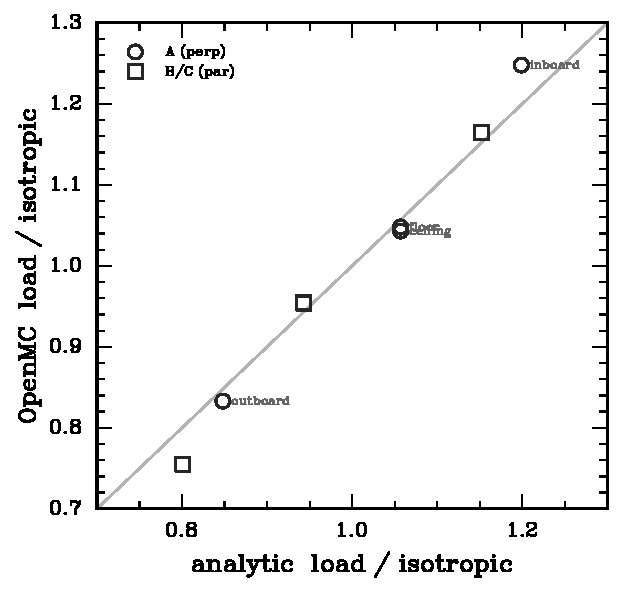
\includegraphics[width=\linewidth]{fig_quasr_validation.pdf}
\end{column}
\begin{column}{0.43\textwidth}
\footnotesize
\begin{itemize}
\item Axisymmetric limit (Schwartz recovery): A-mode midplane $+43\%$/$-22\%$ in the text,
      reproduced as $+39\%$/$-21\%$.
\item Independent cross-check: analytic point-patch vs ray-traced OpenMC on the conformal
      59509 wall agree 0.5--2.3\% by region, per-bin $r=0.91$.
\item Per-wall free-stream error: outboard 1.8\%, floor 0.8\%, ceiling 1.3\%,
      strongly-curved inboard 4.1\%.
\end{itemize}
\end{column}
\end{columns}
\end{frame}

% ============================================================
\begin{frame}{Free Streaming Poloidal NWL Maps}
\begin{columns}[c]
\begin{column}{0.6\textwidth}
\includegraphics[width=\linewidth]{nwl_maps.pdf}
\end{column}
\begin{column}{0.38\textwidth}
\footnotesize
\begin{itemize}
\item $(\theta,\phi)$ NWL on the conformal first wall for QUASR 886079, normalized to the
      mean.
\item Optimal polarization here is $a_2=+0.83$ (strongly parallel-leaning), lowering the
      peaking factor $1.78\to1.49$ (a 16\% reduction).
\item This is the free-streaming pattern; scattering dilutes the modulation.
\end{itemize}
\end{column}
\end{columns}
\end{frame}

% ============================================================
\begin{frame}{How Much Does Polarization Reduce Peaking?}
\begin{columns}[c]
\begin{column}{0.55\textwidth}
\includegraphics[width=\linewidth]{pf_hist.pdf}
\end{column}
\begin{column}{0.43\textwidth}
\footnotesize
\begin{itemize}
\item Ran the peaking-optimal polarization scan in the free-streaming limit for 15 QUASR
      reactor designs spanning shaping amplitude 0.16--1.00.
\item Optimal reduction is weak: 0--16\%, median $\approx4\%$; the 16\% case is an outlier.
\item The optimal $a_2$ itself flips sign across devices ($-0.83$ to $+1.0$): no single
      polarization helps every design.
\item For stellarators, polarization is not a strong peaking-factor lever.
\end{itemize}
\end{column}
\end{columns}
\end{frame}

% ============================================================
\begin{frame}{Predictors Of Steerability}
\footnotesize
Three metrics we test as forecasts of the free-streaming steering benefit:
\begin{itemize}
\item PF$_\mathrm{geo}$ (geometry-only headroom): a transport-free peaking factor from an
      isotropic $1/r^2$ flux proxy $G(\mathbf{w})=\sum_v |\sqrt{g}|_v/|\mathbf{w}-\mathbf{r}_v|^2$
      over source voxels, $\mathrm{PF}_\mathrm{geo}=\max G/\langle G\rangle_A$. High means the
      wall load is geometrically peaked before any physics.
\item Nematic $Q$ (pure plasma shape): $Q=|\langle e^{2i\psi}\rangle|$ over the LCFS
      outward-normal angles $\psi=\arctan2(n_Z,n_R)$. The nematic order of the wall-normal
      director field --- $0$ = orientations isotropic, $1$ = fully aligned.
\item $\varepsilon_\mathrm{eff}$ (helical standoff, my parameter): the non-axisymmetric
      boundary excursion relative to the source-to-wall standoff --- a property of the
      boundary geometry, not $|B|$ quasi-symmetry. Small ($\lesssim0.15$): the analytic
      $P_2$ series is second-order accurate; large ($\gtrsim2$): the series breaks down and
      needs hybrid quadrature. Device 59509: $\varepsilon_\mathrm{eff}\approx0.43$.
\end{itemize}
\end{frame}

\begin{frame}{When Does Polarization Help? (n=15)}
\begin{columns}[c]
\begin{column}{0.55\textwidth}
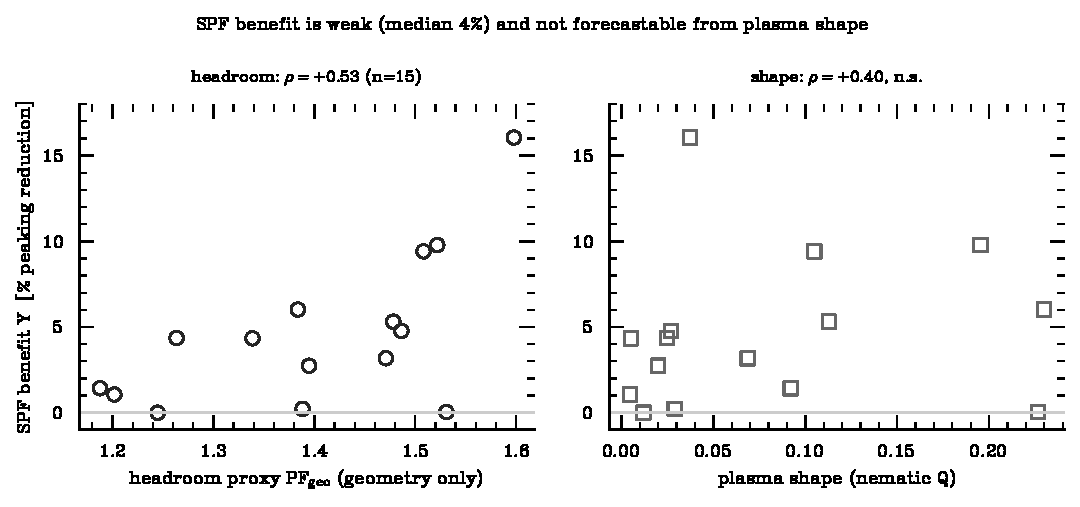
\includegraphics[width=\linewidth]{fig_predictor.pdf}
\end{column}
\begin{column}{0.43\textwidth}
\footnotesize
\begin{itemize}
\item Peaking-factor benefit across 15 conformal-wall QUASR devices is weak everywhere:
      0--16\%, median 4\%.
\item Best predictor is the transport-free headroom PF$_\mathrm{geo}$ ($\rho=+0.53$,
      borderline at $n=15$).
\item Plasma shape (nematic $Q$, $\rho=+0.40$) does not robustly forecast the benefit.
\item Devices drawn from the QUASR database, stratified by symmetry class and field
      period; 30 VMEC solves gave 15 usable conformal maps (aspect ratio 3.3--24, mostly
      quasi-axisymmetric).
\end{itemize}
\end{column}
\end{columns}
\end{frame}

% ============================================================
\begin{frame}{Summary}
Done and verified
\begin{itemize}\footnotesize
\item Native polarized \texttt{Source} plus a 3-D \texttt{StellaratorSource}; the sampler is
      exact ($\chi^2$, KS, moments, $a_2$-linearity).
\item Free-streaming cross-validated against an independent analytic point-patch on real
      QUASR geometry.
\item End-to-end conformal blanket transport with scattering.
\end{itemize}
Limitations
\begin{itemize}\footnotesize
\item Monoenergetic 14.06\,MeV (the \texttt{TokamakSource} energy handling is richer).
\item Constant/toroidal or gridded $\bhat$ only; no depolarization; convex-ish walls.
\item Steering is a source/free-stream effect; scattering dilutes it $\sim3\times$, and the
      peaking-factor benefit is weak for stellarators.
\end{itemize}
\end{frame}

\begin{frame}{Backup: One-Glance Number Table}
\scriptsize
\begin{tabular}{@{}lccccc@{}}
\toprule
mode & $\eta$ & rate & center-stack & inboard NWL$^\ast$ & outboard NWL$^\ast$ \\
\midrule
unpolarized & 0.667 & 1.00 & 1.00 & --- & --- \\
A (perp) & 1.000 & 1.50 & 1.70 & $+40\%\!\to\!+13\%$ & $-20\%\!\to\!-9\%$ \\
B (par) & 0.667 & 1.00 & 0.85 & $-40\%\!\to\!-15\%$ & $+19\%\!\to\!+9\%$ \\
C & 0.333 & 0.50 & 0.42 & (B shape) & (B shape) \\
\bottomrule
\end{tabular}
\vfill
\footnotesize
$^\ast$ Free-Streaming $\to$ full transport. Directional efficiency of the pitched 3-D
field vs pure axisymmetric $\hat\varphi$: $\eta_{\text{dir}}=0.89$. Schwartz recovery
(A midplane): analytic $+43/-22\%$, OpenMC $+39/-21\%$.
\end{frame}

\end{document}
